\documentclass{beamer}

\usepackage{amsmath, amssymb, graphicx, multicol, tikz, array}
\usepackage[absolute,overlay]{textpos}
\usepackage[export]{adjustbox}
\usepackage{pgfplots, pgf-pie}
\usetikzlibrary{positioning}
\usetikzlibrary{calc}
\pgfplotsset{compat=1.17}

% \usepackage{zxjatype}
% \usepackage[ipa]{zxjafont}
% \usepackage{mymacro}

\setbeamerfont*{itemize/enumerate body}{size=\large}
\setbeamerfont*{itemize/enumerate subbody}{parent=itemize/enumerate body}
\setbeamerfont*{itemize/enumerate subsubbody}{parent=itemize/enumerate body}

\usefonttheme{professionalfonts}
\setbeamertemplate{navigation symbols}{}

% --- page number ---
\setbeamertemplate{footline}{%
	\raisebox{10pt}{\makebox[\paperwidth]{\hfill\makebox[7em]{\normalsize\texttt{\insertframenumber/\inserttotalframenumber}}}}%
}

\DeclareMathOperator*{\argmin}{argmin}
\DeclareMathOperator*{\argmax}{argmax}
\DeclareMathOperator{\softmax}{softmax}
\DeclareMathOperator{\ReLU}{ReLU}

\title{Deep learning}
\subtitle{Part 3: Text data}
\author{Matthew Greenberg}
\date{2021.05.03}


\begin{document}

    \begin{frame}
    \maketitle
    \end{frame}

    

    % \begin{center}
    %     \begin{tikzpicture}
    %         \node (topleft) {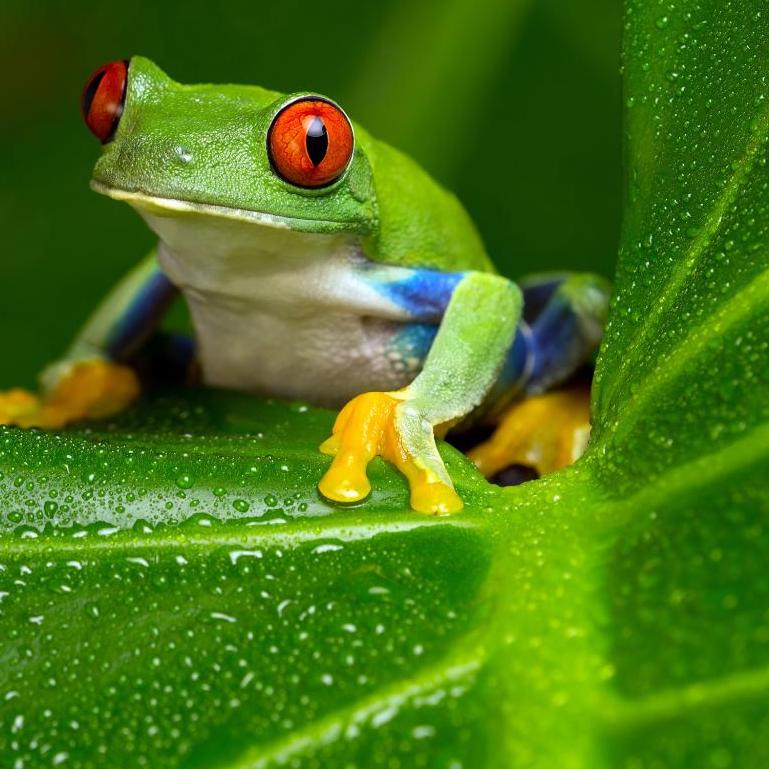
\includegraphics[width=1.5in]{frog-square-top-left.jpeg}};
    %         \node[right=of topleft] (bottomright) {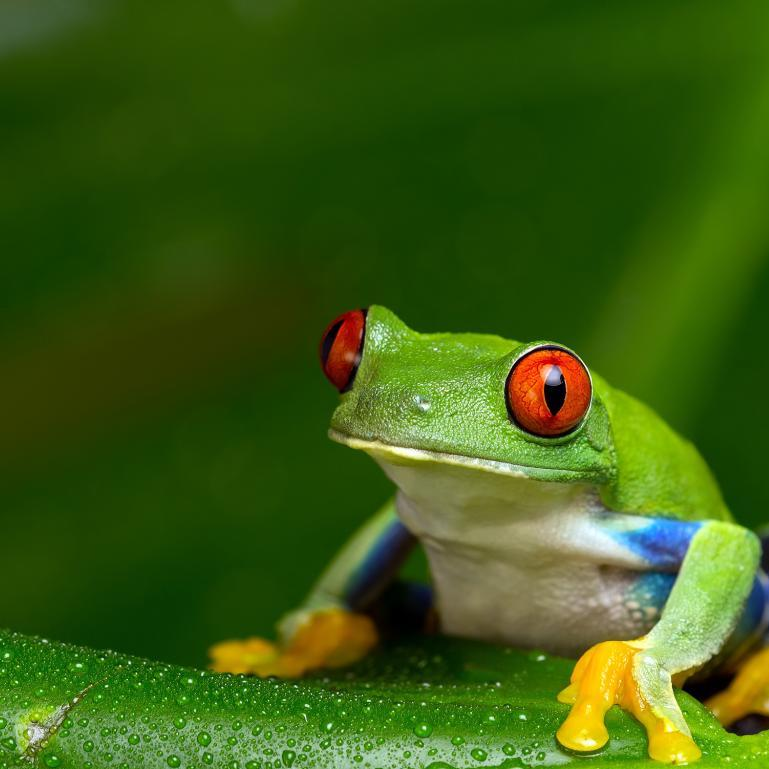
\includegraphics[width=1.5in]{frog-square-bottom-right.jpeg}};
    %     \end{tikzpicture}
    % \end{center}

    \begin{frame}
        \frametitle{}
        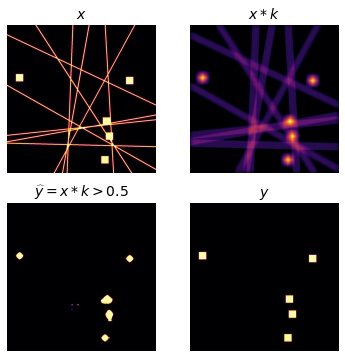
\includegraphics[height=3in]{filter.jpg}
    \end{frame}

    \begin{frame}
        \frametitle{}
        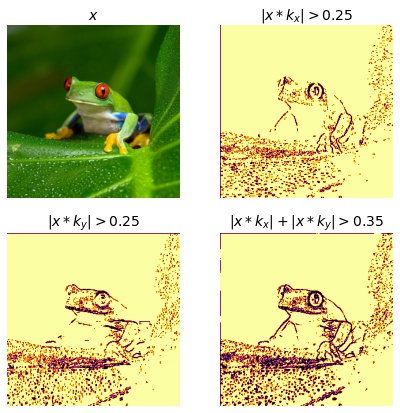
\includegraphics[height=3in]{filtered-frogs.jpg}
    \end{frame}

    \begin{frame}
        \frametitle{}
        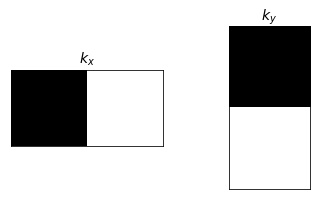
\includegraphics[width=2in]{edge-detectors.jpg}
    \end{frame}

\end{document}
